In order to convert the raw detector readouts to information about a given particle, various sets of reconstruction algorithms are run.
This includes building particle trajectories in the ID, identifying and measuring electrons and muons, and clustering hadronic energy deposits into jets.
A brief overview of these reconstruction methods follow in order to provide context for when these objects are used later in the thesis.

\subsubsection{Track reconstruction}\label{detector:track_reconstruction}
\emph{Track reconstruction} is the process by which a particle's trajectory is reconstructed from the raw measurements (also called \emph{hits}) recorded in the ID.
The ATLAS track reconstruction algorithm~\cite{2017.atlas-track-reconstruction-run2} follows three main steps: clusterization, track finding, and ambiguity solving.

The first step, clusterization, uses hits from the Pixel and SCT detectors.
Neighboring pixels and silicon strips in a sensor are grouped together into clusters using a connected component analysis.
Each cluster represents a \emph{space-point}, or a three-dimensional measurement corresponding to the point where the particle intersected the sensor.
Since the SCT sensors consist of two strip layers on top of each other (as described in Section~\ref{sec:sct}), clusters from each layer combine to form a single space-point.
It is possible to have overlapping clusters from multiple particles in a single sensor, and care is taken that these \emph{merged clusters} are identified and handled accordingly.

Next, track seeds are formed using sets of three space-points.
This number allows for a first momentum estimate to be made while still maximizing the number of track combinations as much as possible.
The impact parameters of a track seed---the distance of closest approach to the collision---are estimated by assuming a perfect helical trajectory in a uniform magnetic field.
In order to ensure the quality of a track seed, criteria on the momentum and impact parameters are imposed as well as a requirement that at least one additional space-point lies along the preliminary trajectory.
Finally, a combinatorial Kalman filter~\cite{1987.kalman-filtering} builds track candidates from the track seeds by incorporating additional space-points lying along the preliminary trajectory.
The filter allows for multpile track candidates to be fit to the same track seed if more than one set of space-points is compatible.

The final step of the reconstruction process is the ambiguity solving.
Each track candidate is processed individually sorted by their \emph{track score}, a metric for quantifying the likelihood that a given track candidate correctly represents the particle's trajectory.
The track score is determined by a number of factors.
Each cluster in the track candidate increases the score by an amount weighted by, for example, the intrinsic resolution of the relevant detector's sensors.
Conversely, if a track candidate passes through a sensor but there is no associated cluster (called a \emph{hole}), the score is reduced.
The $\chi^2$ of the track fit contributes as well in order to promote tracks with high quality fits.
Finally, the logarithm of the momentum adds to the score in order to suppress tracks with incorrectly assigned clusters which typically have low momenta.
A track candidate is rejected by the ambiguity solver if its score is too low, or if it fails to meet a basic set of quality criteria.
If a cluster would be shared by more than one track, at most two tracks are allowed to pass through it.
In this case, preference is given to tracks already passing through the ambiguity solver, which by construction results in the two highest scoring tracks using the shared cluster being kept.

Following this procedure, TRT hits can be incorporated into the track fit through \emph{TRT track extension}~\cite{2008.newt}.
Compatible sets of TRT measurements are found for tracks found in the silicon detectors surviving the ambiguity solving.
The algorithm requires that the original silicon-only track not be modified by the inclusion of the TRT hits; it is simply an extension of the existing track.

What is described above is the \emph{inside-out} reconstruction algorithm; there is also an \emph{outside-in} reconstruction that begins in the TRT.
This algorithm is not covered in detail here, as much of the process is similar to the above.
The general workflow begins with finding track segments in the TRT, constructing the track candidates including the silicon hits, and finally ambiguity solving.

\subsubsection{Electron reconstruction}\label{detector:electron_reconstruction}
Electron reconstruction~\cite{2019.electron-reco-id} uses information from both the ID and the electromagnetic calorimeters.
The characteristic signature of an electron in ATLAS is a charged particle track in the ID matched in $\eta$-$\phi$ to localized clusters of energy deposited in the calorimeter.

Calorimeter cluster candidates are seeded from localized energy deposits according to a sliding-window algorithm~\cite{2008.sliding-window}.
The clusters are a $3\times 5$ ($\eta\times\phi$) rectangle of calorimeter towers with a total transverse energy greater than $2.5\gev$.
In the event that two clusters overlap, if the clusters' $\et$ vary by more than 10\% the highest $\et$ cluster is kept, otherwise the candidate with the highest $\et$ in the central tower is kept.
The ID tracks are those generated using the algorithm detailed above in Section~\ref{detector:track_reconstruction}, and tracks with a nearby calorimeter cluster are re-fit using a Gaussian-sum filter~\cite{2003.gsf} designed to take into account bremsstrahlung effects.

To reconstruct the final electron candidate, the refit track and the cluster are subject to the final matching criteria:
\begin{equation}
  \begin{gathered}
  |\eta_{\textrm{cluster}} - \eta_{\textrm{track}}| < 0.05 \\
  \textrm{and}\\
   -0.10 < q\times \Delta\phi_{\textrm{cluster, track}} < 0.05 \textrm{\ \ \ or\ \ \ }-0.10 < q\times \Delta\phi_{\textrm{res}} < 0.05
  \end{gathered}
\end{equation}
where $q$ is the charge of the track and $\Delta\phi_{\textrm{res}}$ is the azimuthal separation between the cluster position and the track after rescaling its momentum to the energy of the cluster.
If multiple tracks satisfy the above criteria, the primary track is selected by an algorithm that takes into account the center of each cluster relative to the parameters of the candidate track.
Finally, the clusters are reconstructed about the seed cluster using a larger window size, $3\times 7$ in the barrel and $5\times 5$ in the endcaps, and the energy is calibrated to the original electron energy using techniques described in~\cite{2014.electron-calibration-run1, 2018.electron-calibration-run2}.

\paragraph*{Electron identification}
To determine whether an electron candidate is a signal electron or background object, an identification criteria (ID) is implemented, covered in more detail in~\cite{2019.electron-reco-id, 2016.electron-performance-13tev}.
Electron ID is performed using a multivariate likelihood technique (LH) that simultaneously evaluates a list of measurements of an electron candidate, including both tracking and clustering information.
To cover the different requirements of physics and performance studies, four different likelihood working points are constructed corresponding to increasing thresholds for the LH discriminant: \tt{VeryLooseLH}, \tt{LooseLH}, \tt{MediumLH}, and \tt{TightLH}.
Each successive working point is a subset of its predecessors.
The efficiencies of the \tt{LooseLH}, \tt{MediumLH}, and \tt{TightLH} working points as a function of electron $\et$ are shown in Figure~\ref{fig:electron_id_efficiency}.

\begin{figure}[htbp]
  \centering
  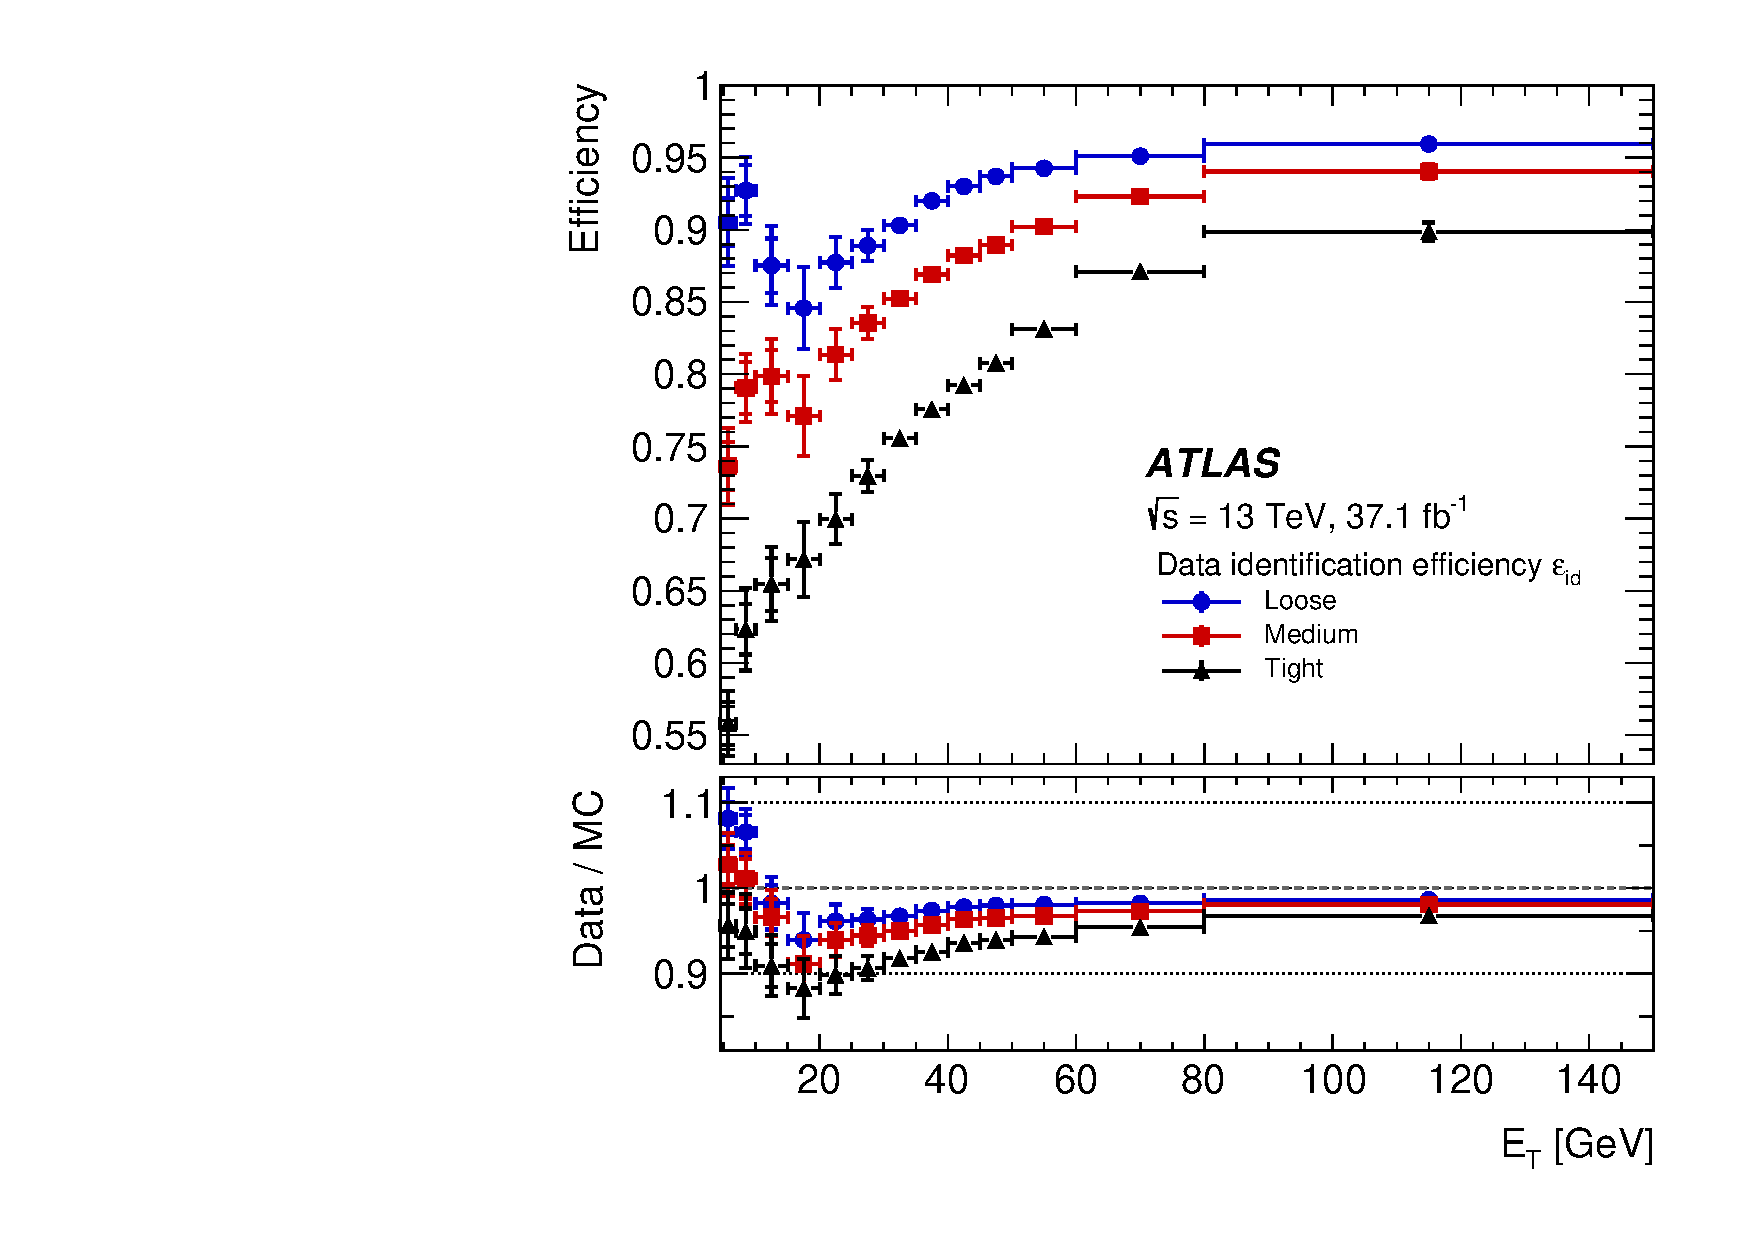
\includegraphics[width=.6\textwidth]{figs/detector/electron_id_efficiency}
  \caption[Measured LH electron ID efficiencies in $Z\rightarrow ee$ events for the \tt{LooseLH} (blue), \tt{MediumLH} (red), and \tt{TightLH} (black) working points as a function of electron $\et$. The bottom panel shows data-to-simulation ratios.]{Measured LH electron ID efficiencies in $Z\rightarrow ee$ events for the \tt{LooseLH} (blue), \tt{MediumLH} (red), and \tt{TightLH} (black) working points as a function of electron $\et$. The bottom plot shows data-to-simulation ratios. Plot taken from~\cite{2019.electron-reco-id}.}
  \label{fig:electron_id_efficiency}
\end{figure}

\paragraph*{Electron isolation}
Signal electrons, such as those from the decay of a $W$ boson, tend to have little detector activity nearby in both the ID and the calorimeters.
Background electrons, such as those from photon conversions or jets, are often produced in association with other particles.
To take advantage of this, variables are consructed to quantify the amount of activity within a cone of a specified radius in $\Delta R$ about an electron---one track-based and a second calorimeter-based.

The track-based isolation consists of the sum of the transverse momentum of tracks with $\pt > 1\gev$ that satisfy basic quality requirements within a cone of $\Delta R < 0.2$ about an electron (not including the electron itself).
Additionally, additional particles from bremsstrahlung radiation are considered part of the original electron and are subtracted from the isolation cone.

Calorimeter isolation is a bit more difficult due to the size of the energy deposits relative to the cone size, as parts of an energy cluster can lie outside of the cone.
As such, topological clusters~\cite{2017.topo-clustering} (topo clusters) are seeded by calorimeter cells with deposited energy greater than four times the expected noise-level of that cell.
The cluster is then expanded incorporating electromagnetic and hadronic cells with an energy greater than two times the noise-level until no adjacent clusters remain satisfying the requirement.
The isolation cone is then the sum of the $\et$ of all positive-energy topo clusters whose barycenters fall within a cone of radius $\Delta R < 0.2$.
The electron's energy is subtracted by removing the cells within a rectangle around the electron.

Four isolation working points are defined targeting specific values of isoation efficiency.
\tt{Loose} and \tt{LooseTrackOnly} target a fixed efficiency value across the $\pt$ and $\eta$ spectrum of the electrons, with the latter not applying a cut on calorimeter isolation.
\tt{Gradient} and \tt{GradientLoose} target a $\pt$-dependent fixed efficiency that is uniform in $\eta$.
The efficiencies for these working points as a function of electron $\et$ are shown in Figure~\ref{fig:electron_iso_efficiency}.
Additional working points are provided that instead use fixed values for the relative track and calorimeter isolation cuts.

\begin{figure}[htbp]
  \centering
  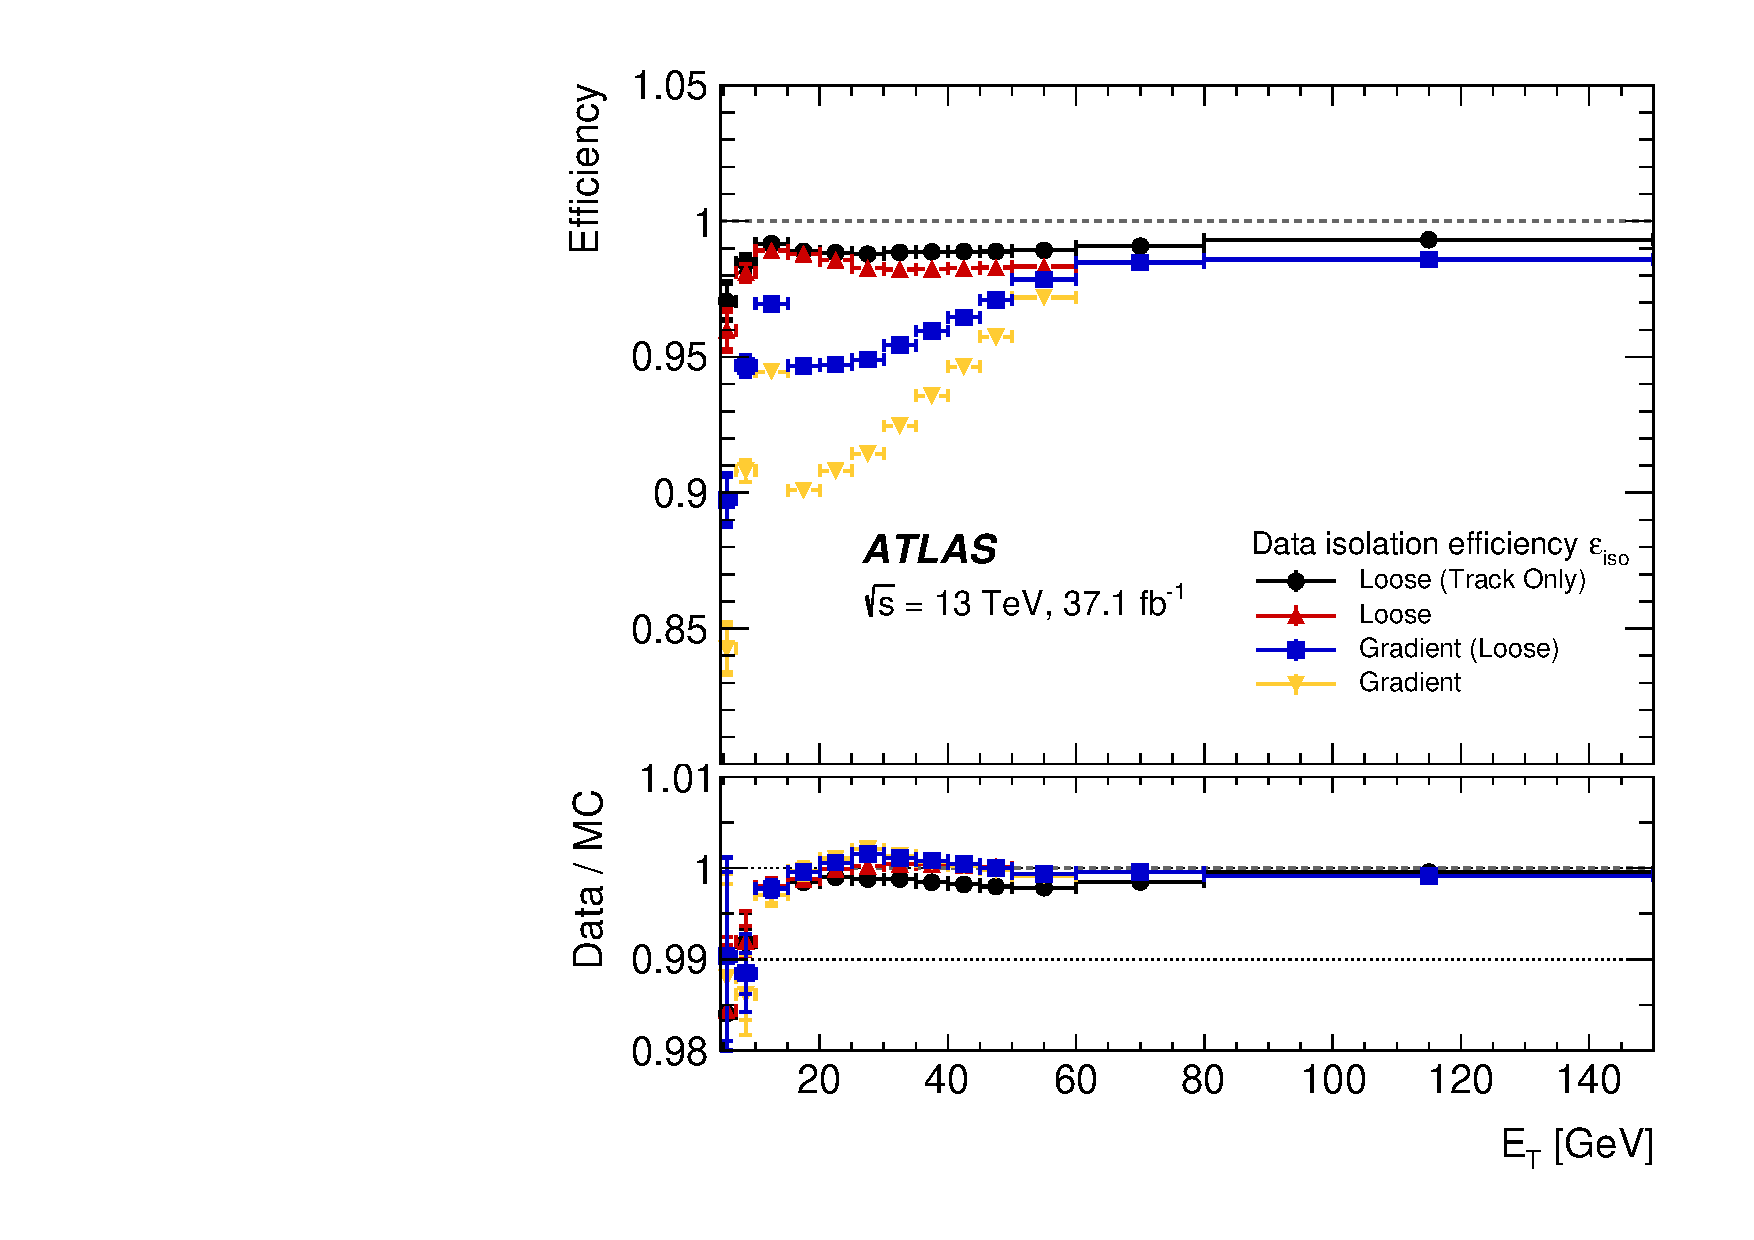
\includegraphics[width=.6\textwidth]{figs/detector/electron_iso_efficiency}
  \caption[Measured isolation efficiencies for the \tt{LooseTrackOnly} (black), \tt{Loose} (red), \tt{GradientLoose} (blue), and \tt{Gradient} (yellow) working points as a function of electron $\et$.  The bottom panel shows data-to-simulation ratios.]{Measured isolation efficiencies for the \tt{LooseTrackOnly} (black), \tt{Loose} (red), \tt{GradientLoose} (blue), and \tt{Gradient} (yellow) working points as a function of electron $\et$.  The bottom panel shows data-to-simulation ratios.  Plot taken from~\cite{2019.electron-reco-id}.}
  \label{fig:electron_iso_efficiency}
\end{figure}

\subsubsection{Muon reconstruction}\label{detector:muon_reconstruction}

\subsubsection{Jet reconstruction}\label{detector:jet_reconstruction}
